\section{Theoretische Grundlagen}

%Zerfallskaskaden
%Zufällige Koinzidenzen

\subsection{$\alpha$-Zerfall}

Zerfällt ein sogenannter Mutterkern $_Z^AX$ in einen Tochterkern $_{Z-2}^{A-4}Y$ und ein $He^{2+}$-Ion so spricht man von $\alpha$-Zerfall. Das $He^{2+}$-Teilchen wird $\alpha$-Teilchen genannt. Die Emission von $\alpha$-Teilchen ist ein quantenmechanischer Prozess, der durch das Tunneln des $\alpha$-Teilchens durch die Potentialbarriere des Coulombpotentials des Kerns ermöglicht wird. $\alpha$-Teilchen zeigen ein diskretes Spektrum und sind monochromatisch.

\subsection{$\beta$-Zerfall}

Man unterscheidet beim $\beta$-Zerfall zwischen $\beta^+$- und $\beta^-$-Zerfall. Der $\beta^+$-Zerfall ist die Umwandlung eines Protons in ein Neutron mit Emission eines Positrons und eines Elektronenneutrinos:

$$ \beta^+: p^+ \rightarrow n^0 + e^+ + \nu_e $$

Der $\beta^-$-Zerfall hingegen, ist die Umwandlung eines Neutrons in ein Proton, unter Emission eines Elektrons und eines Elektron-Antineutrinos:

$$ \beta^-: n^0 \rightarrow p^+ + e^- + \bar \nu_e $$

Der $\beta^+$-Zerfall ist nur möglich für Protonen in einem Kern, da durch die Bindungsenergie die für den Prozess nötige Energie aufgebracht werden kann.

Als weitere Art des $\beta$-Zerfall zählt man noch den Elektroneneinfang (EC, \emph{electron capture)}. Dieser kann stattfinden, wenn ein Elektron der untersten Schale (K-Schale), wegen dessen Aufenthaltswahrscheinlichkeit im Kern, vom Kern eingefangen wird und mit einem Proton zu einem Neutron wird unter Emission eines Elektronenneutrinos:

$$ EC: p^+ + e^- \rightarrow n^0 + \nu_e $$

Der Elektroneneinfang gewinnt mit größeren Kernzahlen an Bedeutung, da dann die Aufenthaltswahrscheinlichkeit im Kern immer größer wird.

\subsection{$\gamma$-Strahlung}

Beim $\alpha$- und $\beta$-Zerfall gehen die Mutterkerne immer mit bestimmten Wahrscheinlichkeiten in verschiedene Zustände der Tochterkerne über. Letztere zerfallen innerhalb einer sehr kurzen Zeit ($\sim 10^-9 bis 10^-12 s$) in den Grundzustand und emittieren dabei ein Photon, genannt $\gamma$-Quant. Dieses $\gamma$-Quant wird entweder direkt vom Kern emittiert oder kann folgende Prozesse auslösen:

\subsubsection{Innere Konversion}

Die Energie des Kerns geht an ein Hüllenelektron, welches dadurch das Atom mit der verbleibenden Energie als kinetische Energie verlässt. Diese Elektronenlücke wird durch ein Elektron aus einer höheren Schale ersetzt, welches diesen Energieverlust durch ein Photon (bei schweren Elementen) oder den Auger-Effekt (bei leichten Elementen) kompensiert.

\subsubsection{Der Auger-Effekt}

Falls dieses oben erklärte Elektron dieses Loch füllt, kann es sein, dass die überschüssige Energie wiederum an ein Elektron abgegeben wird, welches dadurch das Atom verlässt und damit ein zweites Loch im Atom hinterlässt.


\subsection{Wechselwirkung von Photonen mit Materie}

\subsubsection{Das Absorptionsgesetz}

Ein Photonenstrahl der einfallenden Intensität $I_0$ nimmt exponentiell mit der Dicke x einer durchquerten Materieschicht an Intensität ab. Es gilt also:

$$ I = I_0\cdot e^{-\mu x} $$

wobei $\mu$ der mediumabhängige (und photonenenergieabhängige) Absorptionkoeffizient ist. $\mu$ lässt sich als Summe der Absorptionskoeffizienten aller möglichen Wechselwirkungen von Photonen mit Materie schreiben, nämlich des Photoeffekts, des Compton-Effekts und der Paarbildung.

$$\mu = \mu_{Ph.} + \mu_{C} + \mu_{PB} $$

\subsubsection{Der Photoeffekt}

\begin{figure}[H]
	\begin{minipage}{0.6\textwidth}
	\centering 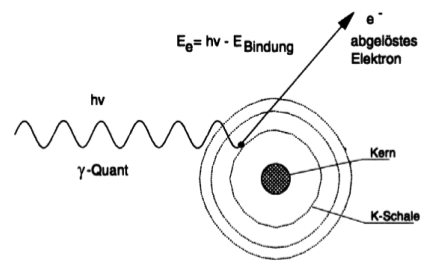
\includegraphics[width=\textwidth]{Bilder/Photoeffekt.png}
	\caption{Photoeffekt}
	\end{minipage}
	\begin{minipage}{0.4\textwidth}
	Wenn ein $\gamma$-Quant ein Elektron aus der Atomhülle herausschlägt, spricht man vom Photoeffekt. 	Dieser Effekt tritt also nur an gebundenen Elek\-tro\-nen auf. Die Energie des Photons geht zum größten Teil 	auf das Elektron, ein Teil wird jedoch als Rückstoßenergie vom Atom aufgenommen. Die 				Ab\-sorp\-tions\-wahrscheinlichkeit ist am größten in der K-Schale, also näher beim Kern. Der Photoeffekt 	dominiert gegenüber den anderen Effekten vor allem bei großen Atomen und Energien unter 100keV des	Photons. Nach dem Ablösen des Elektrons strahlt das ionisierte Atom die Bindungsenergie wieder ab.
	\end{minipage}
\end{figure}

\subsubsection{Der Compton-Effekt}

\begin{figure}[H]
	\begin{minipage}{0.4\textwidth}
	Trifft ein Photon auf ein leicht gebundenes oder freies Elektron, so wird das Photon nicht ganz absorbiert, sondern gibt einen Teil seiner Energie an das Elektron ab und wird selbst gestreut. Durch die Streuung verliert das Photon somit an Energie, d.h. die Frequenz des gestreuten Quants ist kleiner. Der Compton-Effekt dominiert bei Energien zwischen 100 keV und einigen MeV.
	\end{minipage}
	\begin{minipage}{0.6\textwidth}
	\centering 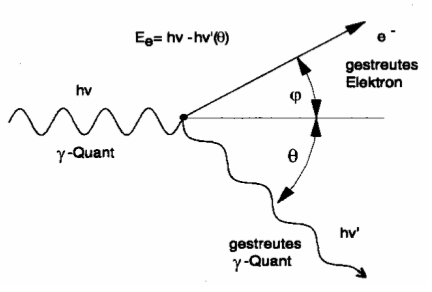
\includegraphics[width=\textwidth]{Bilder/Comptoneffekt.png}
	\caption{Comptoneffekt}
	\end{minipage}

\end{figure}

\subsubsection{Die Paarbildung}

\begin{figure}[H]
	\begin{minipage}{0.5\textwidth}
	\centering 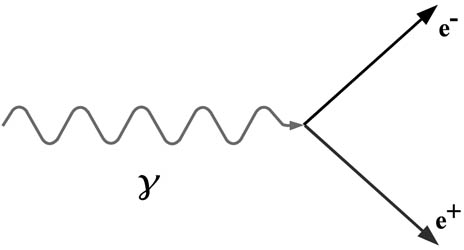
\includegraphics[width=\textwidth]{Bilder/Paarbildung.jpg}
	\caption{Paarbildung}
	\end{minipage}
	\begin{minipage}{0.5\textwidth}
	Hat der $\gamma$-Quant mindestens die doppelte Ruheenergie eines Elektrons, also 1.022 MeV, so kann dieses im Feld eines Atomkerns (Stoßpartner für die Energie-Impuls-Erhaltung) ein Elektron-Positron-Paar erzeugen. Das Positron kann in Anwesenhait von Materie nicht frei existieren und wird abgebremst und annihiliert mit einem Elektron zu 2 bis 3 $\gamma$-Quanten. Im wahrscheinlicheren Fall zweier Quanten, erhalten diese jeweils eine Energie von 511 keV und bewegen sich in einem Winkel von 180$^\circ$ relativ zueinander (wegen Impulserhaltung).
	\end{minipage}
\end{figure}

\subsection{Der Szintillationszähler}

\begin{figure}[H]
	\centering 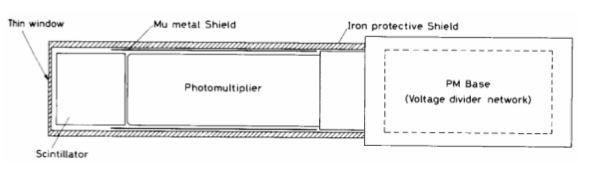
\includegraphics[width=\textwidth]{Bilder/Szinti.png}
	\caption{Schema eines Szintillationszählers}
\end{figure}

Ein Szintillationszähler ist ein Gerät zum Nachweis ionisierender Strahlung. Die vom Quant abgegebene Energie wird in Licht verwandelt und von einem Photomultiplier verstärkt. Dieses Licht ist proportional zur Energie des Quants. Man unterscheidet zwischen organischen und anorganischen Szintillatoren. Bei dem organischen werden einzelne Moleküle angeregt, welche Messbare Quanten emittieren. Beim anorganischen entstehen diese in einem Kristallgitter:

\begin{figure}[H]
	\begin{minipage}{0.45\textwidth}
	Der organische Szintillator selber ist ein NaI-Kristall mit Tl-Aktivatorzellen. Das Bändermodell erlaubt eine einfache Beschreibung des Verhaltens. Nämlich befinden sich bei tiefen Temperaturen alle Elektronen des Kristalls im sogenannten Valenzband. Absorbieren diese Elektronen energiereiche Strahlung, z.B. durch $\gamma$-Quanten (v.a. Photoeffekt), so werden diese angeregt und steigen auf höhere Energieniveaus. Reicht die Energie aus, so werden die Elektronen ins Leitungsband gehoben. Falls sie nicht groß genug ist um das Elektron vom Valenzband ins Leitungsband zu heben, so können sogenannte Exzitonen entstehen, lose gekoppelte Elektron-Loch-Paare (siehe Bild). Die Exzitonen, können sich genau so wie die Leitungsband-Elektronen frei im Kristall bewegen und können unter Emission 
	\end{minipage}
	\begin{minipage}{0.55\textwidth}
	\centering 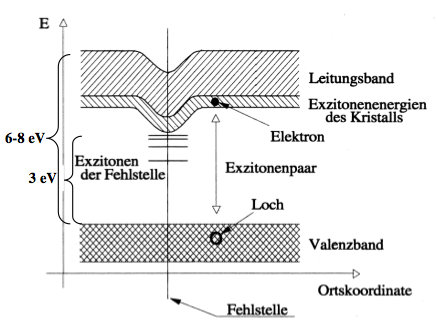
\includegraphics[width=\textwidth]{Bilder/Bandmodell.png}
	\caption{Bändermodell beim NaI:Tl$^+$}
	\end{minipage}
\end{figure}
eines Photons wieder in den Grundzustand zurückkehren. Eintreffende $\gamma$-Quanten haben Energien im Bereich von 0.1 bis 1 MeV, regen also mehrere hundert Elektronen gleichzeitig an. Wenn diese Elektron-Loch-Paare rekombinieren, entstehen neue Photonen, welche in den Photomultiplier geraten und dort verstärkt werden. Die Dotierung verformt lokal das Leitungsband und da diese Photonen vor allem an den Tl-Störstellen rekombinieren, reicht ihre Energie nicht aus um andere Elektronen ins Leitungsband anzuregen, somit können die Photonen nicht wieder vom Kristall absorbiert werden.

Im Photomultiplier (PM) angekommen, treffen die Photonen auf eine Kathode, an der sie per Photoeffekt Elektronen herausschlagen, welche wegen einer anliegenden Spannung zu einer Dynode beschleunigt werden. An dieser Dynode werden dann wiederum Elektronen herausgeschlagen, und zur nächsten beschleunigt und so weiter. Die Anzahl an Elektronen wird somit an jeder Dynode vervielfacht, so dass das Signal verstärkt wird. Letzteres wird an einer Anode in proportionale Stromimpulse umgesetzt.

\subsection{Versuchsaufbau}

\begin{figure}[H]
\centering 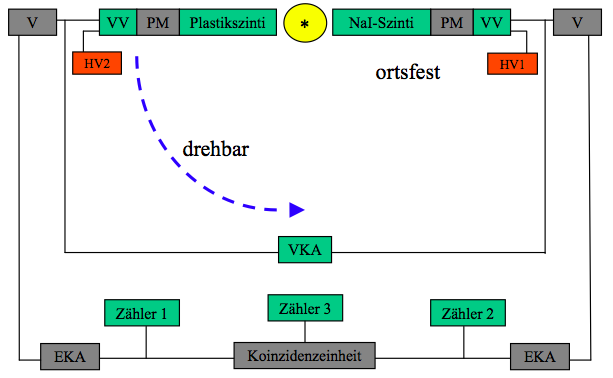
\includegraphics[width = \textwidth]{Bilder/Aufbau.png}
\caption{Versuchsaufbau}
\end{figure}

* ist hier das radioaktive Präparat. Die verschiedenen Abkürzungen werden in der Theorie unter \emph{Signalverstärkung} definiert und die Funktionsweise aller Komponenten erläutert.

\subsection{Signalverstärkung}

\subsubsection{Der Vorverstärker (VV)}

Der Vorverstärker integriert die vom Photomultiplier ankommenden Stromimpulse über eine bestimmte Zeit ($\sim$ 100 ns) und gibt so eine proportionale Ausgangsspannung heraus, dessen Amplitude gemessen werden kann.

\subsubsection{Der Hauptverstärker (HV)}

Am Hauptverstärker können gleichzeitig die weitere Verstärkung des Signals, sowie dessen \emph{shaping time} eingestellt werden. Die Verstärkung kann die Amplitude des Signals auf einige Volt bringen.  Die \emph{shaping time} ist die Zeit, in der das Signal differenziert und integriert wird, um eventuelle Fehler und Schwankungen herauszufiltern. Der Hauptverstärker besitzt einen unipolaren und einen bipolaren Ausgang, wobei der bipolare die Differentiation des unipolaren ist. Außerdem kann man einen Delay zwischen beiden Signalen einstellen und die Polarität ändern.

\subsubsection{Der Vielkanalanalysator (VKA)}

Der Vielkanalanalysator verteilt die Ausgangsimpulse des Hauptverstärkers je nach Spannungshöhe auf verschiedene Kanäle (hier 8192 Kanäle). Der Kanalinhalt wird bei jedem Ereignis der bestimmten Spannungshöhe um 1 erhöht, was ermöglicht die Anzahl der Impulse einer bestimmten Spannung zu messen. Die Kanal-Energie-Abhängigkeit kann man dann durch bekannte Energien (vgl. 511keV-Linie) bestimmt werden.

\subsubsection{Der Einkanalanalysator (EKA)}

Der Einkanalanalysator wird mit dem bipolaren Ausgang des Hauptverstärkers verbunden. Im EKA kann man einstellen, welche Signale man messen will. Man kann dazu eine minimale und eine maximale Schwelle (\emph{lower und upper level}) einstellen, die erlauben, dass nur Signale registriert werden, deren Energie in dem Bereich zwischen beiden Schwellen liegt. Wird ein Signal registriert, so wird ein messbarer Puls erzeugt. Am EKA kann man außerdem noch die Verzögerung (\emph{Delay}) zwischen beiden Signalen und das \emph{Gate} einstellen. Ein \emph{Gate} ist ein einstellbarer Zeitraum, in dem ein Signal registriert werden soll. Liegt das Signal außerhalb des eingestellten \emph{Gates}, wird es nicht registriert. 

\subsubsection{Die Koinzidenzeinheit}

Bei der Koinzidenzmessung wird gemessen, ob zwei $\gamma$-Quanten gleichzeitig in beiden Szintillationszählern ankommen. Wenn zwei $\gamma$-Quanten innerhalb einer fest eingestellten kurzen Zeitspanne $\Delta t$ in beiden Szintillationszählern ankommen, so registriert ein Zähler einen Count. In unserem Versuch werden die Koinzidenzen für verschiedene Winkel zwischen den beiden Szintillationszählern gemessen.

















